% !TEX root = ./Thesis - combined.tex

\chapter{Introduction}\label{Introduction}

Microfluidics is a broad term that covers a wide variety of research, it is characterised by
the analysis of small volumes of liquids usually nL to $\mu$L, in doing so, it offers numerous benefits
such as: a reduction in the materials used in experiments leading to lower costs and less waste; a high
level of control over the microenvironment; and ease of parallelisation and automation.
Microfluidics chiefly uses Lab-on-a-chip (LoC) devices, or micro total analysis
systems (µTAS), to perform experiments. These devices, or systems, are intended for the of scaling down of
laboratory functions to a chip-format, the sizes of which range from a few mm$^2$ to a few cm$^2$.
Currently, NMR spectroscopy is not widely utilised in microfluidic devices, or experiments, and could be
used to provide extra information on the system of interest. Its non-invasive, non-destructive nature means that it
can also be used in conjunction with existing methods of analysis in microfluidics such as fluorescence spectroscopy.
As NMR leaves the sample unperturbed, this makes it an ideal candidate for \textit{in situ} monitoring of
living systems.

The goal of the work presented here is to incorporate functional microfluidic experiments with high
resolution NMR spectroscopy, in such a way that the validity of either technique, microfluidic or magnetic
resonance, remains intact. In this approach, microfluidic capability is preserved by utilising a design
that, whilst constrained by size and shape, has freedom to house a wide variety of chip designs which enable
a host of applications, a few of these are shown in \fig{fig:DifferentChips}. This means that functional
microfluidics can be performed, and coupled, with high resolution NMR spectroscopy. In doing so, not only
could NMR become a more widely used tool in the microfluidic toolbox, it would also make a valuable
attachment to existing tools.

High resolution NMR spectroscopy itself requires an extremely homogenous magnetic field, this means that
any device capable of combining microfluidics and NMR should seek to preserve the homogeneity. This combination
however, is not without significant challenges. Firstly, a probe capable of µNMR must
be designed with comparable performance to existing probes, to maintain validity, and work with existing
magnets and spectrometers. Secondly, the chip, and any functionality it possesses, must fit in the bore of
the magnet which is typically around 38 mm in diameter. This chip should also couple to the probe in a
removable way to enable parallelisation of experiments, preserving one of the key attributes of microfluidics.
Thirdly, the materials used in construction should be non-magnetic wherever possible and the use of magnetic
parts should be kept to a minimum. When designing experiments, the magnetic susceptibilities of solutions and
chip material should also be considered, as these need to be as closely matched as possible in order to preserve
spectral resolution (a solution for when this is not the case is discussed in chapter \ref{Chapter:Droplets}).


\begin{figure}
  \begin{center}
  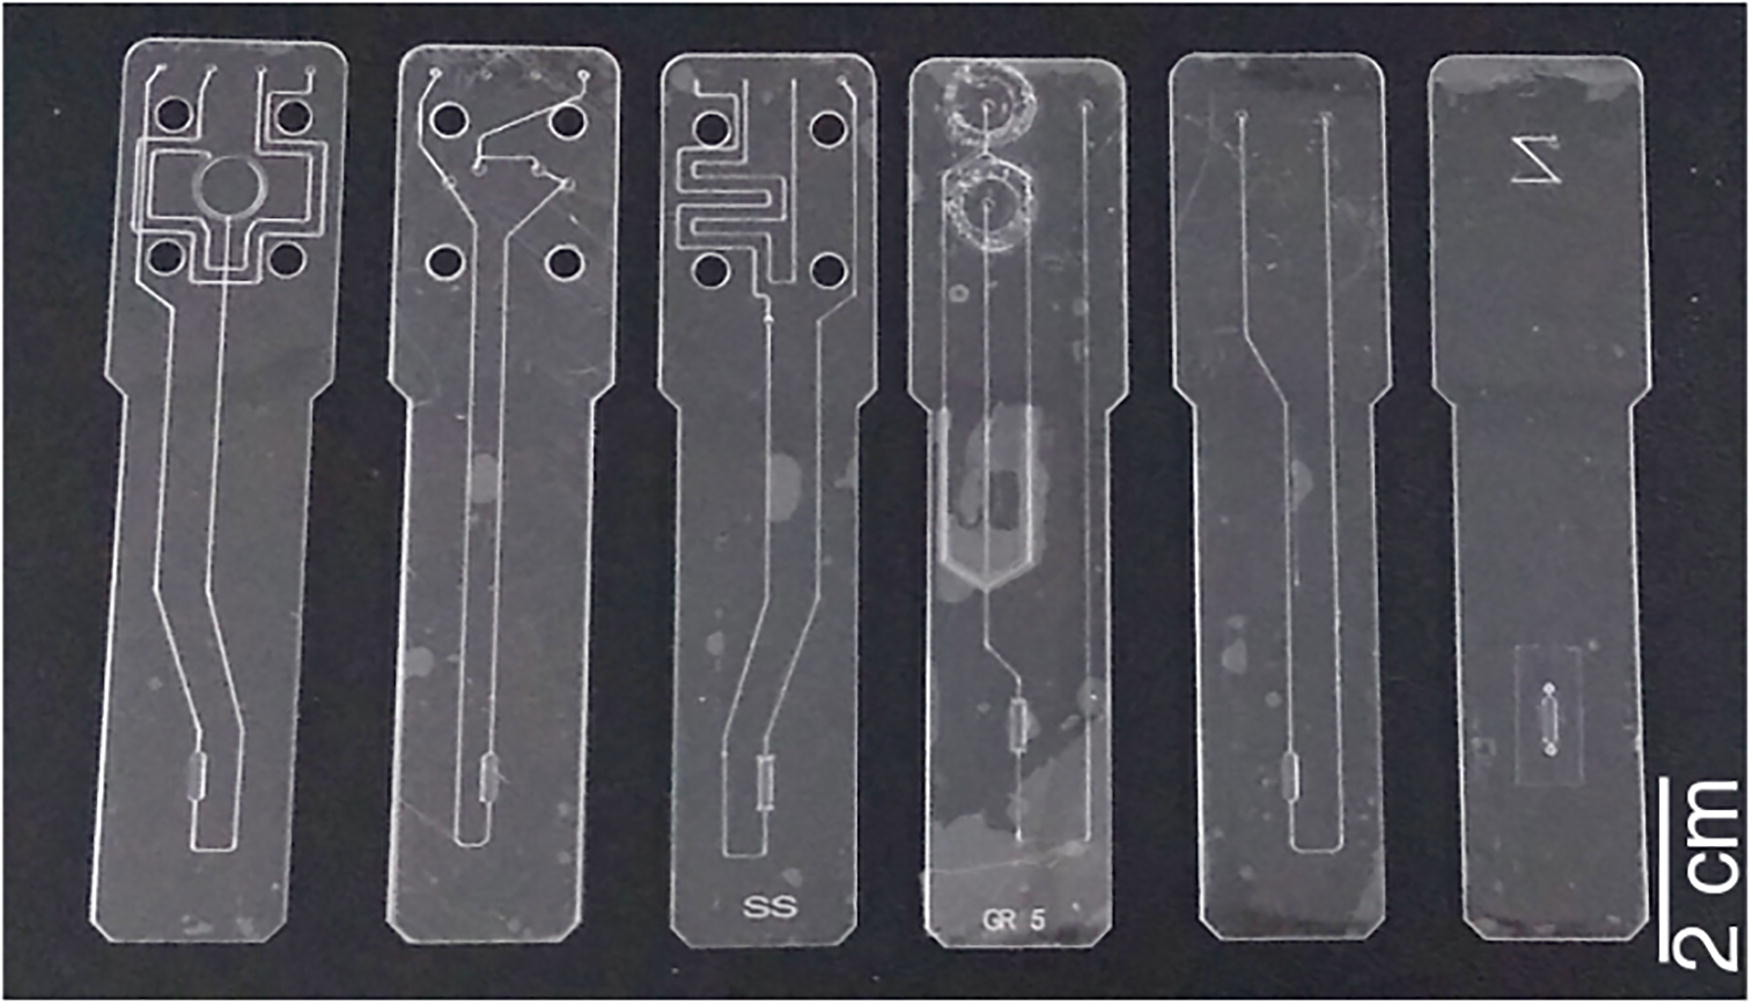
\includegraphics[width=\textwidth]{MVChips.jpg}
  \end{center}
  \caption{Microfluidic devices developed for this work, as well as for other applications in microfluidic
  NMR. From the left: A device for perfusion culture of a tissue slice on chip; capable of peristaltic
  pumping; hydrogenation on a chip; droplet generation; simple sample chamber filler; 2D/3D cell culture
  device. Figure taken from \citep{sharma2019modular}.}
  \label{fig:DifferentChips}
\end{figure}

By combining these two fields, and harnessing the 'best of both worlds' approach,
new insight and analysis is available. Having quantitative, system-level information, in a
a single or just a few scans could benefit a wide variety of experiments. Enabling microfluidic
NMR also provides the oppurtunity to scan mass-limited samples, such as those commonly found in
ligand binding reactions \citep{Finch:2016gv} or macrocyclic chemistry \citep{RN81}.
